\documentclass[11pt]{report}
\renewcommand{\baselinestretch}{1.5}


% Declaração dos pacotes
\usepackage[utf8]{inputenc}
\usepackage[T1]{fontenc}
\usepackage{graphicx}
\usepackage[portuguese]{babel}
\usepackage{graphicx}
\usepackage[affil-it]{authblk} % Usado para meter nome da escola
\usepackage{eurosym} % Usado para o €
\usepackage{url} % URL



% CAPA
\title{\textbf{\textit{Desenvolvimento de uma estação meteorológica em bare-metal e RTOS. }\\
		\large1º Trabalho prático de
		Sistemas Embebidos e de Tempo Real }}
			
				
\author{Rúben Guimarães nº11156\\ Kyrylo Yavorenko nº10355 }

\affil{Escola Superior de Tecnologia, IPCA \\
	Barcelos}	
	
		
\date{06 de Maio de 2018}


\begin{document}

\maketitle




% Indice
\tableofcontents


% Introdução
\chapter*{Introdução}
\addcontentsline{toc}{chapter}{Introdução}


O trabalho prático abordado neste relatório foi desenvolvido no âmbito da unidade curricular Sistemas Embebidos e de Tempo Real do curso de Engenharia de Sistemas Informáticos, lecionada pelo docente António Moreira. O docente desafiou os alunos a aplicarem os conceitos de programação de sistemas embebidos e de sistemas embebidos adquiridos durante o decorrer da unidade curricular. Desenvolvendo um projeto onde o desenvolvimento estivesse divido em duas partes (baremetal e e usando o sistema operativo FreeRTOS) e que adquirisse de diversas fontes de sinais analógicos e digitais para poder replicar o funcionamento de uma estação meteorológica.


\clearpage



% Resumo
\chapter*{Resumo}
\addcontentsline{toc}{chapter}{Resumo}

Neste trabalho desenvolvemos uma pequena estação meteorológica recorrendo a plataforma de prototipagem eletrónica open-source Arduino. Esta estação consiste num conjunto de sensores que obtém dados sobre o estado do tempo que depois são enviados para o Arduino para serem processados e por fim são mostrados ao utilizador quer através de um lcd de 16x2 quer através da consola do IDE do Arduino.


\clearpage


% Objectivos
\chapter*{Objectivos}
\addcontentsline{toc}{chapter}{Objectivos}

Os objetivos definidos para o projecto pelo docente foram:

\begin{itemize}
\item Desenvolvimento de um programa usando a tipologia baremetal.
\item Desenvolvimento de um programa usando o sistema operativo FreeRTOS usando 3 tasks.
\item Utilizar os seguintes sensores:
\begin{itemize}
\item Sensor de água.
\item 3 LDR's para calcular a posição do sol.
\item Sensor de humidade.
\item Dois sensores de temperatura (para o ar e o solo).
\item Barómetro.
\item Anemômetro 
\end{itemize}
\end{itemize}


\clearpage


% Arquitectura
\chapter*{Arquitectura}
\addcontentsline{toc}{chapter}{Arquitectura}

Podemos consultar na figura seguinte um diagrama com a arquitectura do projecto.


\begin{figure} [!h]
\centering
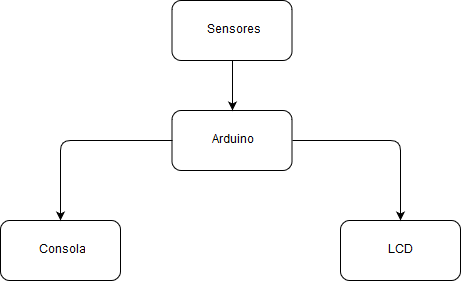
\includegraphics[width=\textwidth]{Prints/arquitectura.png}
\caption{Diagrama da arquitectura do projecto}
\label{Rotulo}
\end{figure}


\clearpage


% Recursos usados no projecto
\chapter*{Recursos usados no projecto}
\addcontentsline{toc}{chapter}{Recursos usados no projecto}

Para o desenvolvimento do projecto foram utilizados os seguintes recursos:

\textbf{Software:}
\begin{itemize}
\item \textit{Arduino IDE 18.5} para o desevolvimento do codigo usado.
\item \textit{GitHub Desktop} para atualizar o repositorio com o codigo do projecto.
\item \textit{Fritzing 0.9.3b} para criar os prototipos dos esquema do projecto.

\end{itemize}

\textbf{Hardware:}
\begin{itemize}
\item \textit{Arduino Mega 2560,} placa que contem o microcontralador que controla tudo o nosso projecto.
\item \textit{DHT11,} sensor usado para obter leituras da humidade e da temperatura do ambiente.
\item \textit{DS18B20,} sensor à prova de água usado para obter temperaturas de água.
\item \textit{BMP180,} sensor que obtem leituras da pressão atmosferica e da temperatura ambiente, com os valores obtidos conseguimos fazer uma estimativa da altitude.
\item \textit{Water Sensor,} sensor usado para saber se existe água ou não.
\item \textit{Buzzer,} usado para dar um feedback sonoro caso seja detectada água no sensor de água.
\item \textit{QTR-8RC,} sensor usado para contar as rotações por minuto de um cata-vento.
\item \textit{LCD 16x2,} usado para mostrar os valores obtidos pelos sensores.
\item \textit{Light Dependent Resistor,} usado para descobrir qual dos lados (este, sul ou oeste) o sol de encontra.
\item \textit{Breadboard,} usada para montar o circuito.
\item \textit{Diversas resistencias,} usadas para proteger componentes ou para servirer de pull-up.
\item \textit{Diversos fios,} usados para efetuar as ligações entre componetes, breadboard e o arduino.

\end{itemize}



% Esquema do projecto
\chapter*{Esquema do projecto}
\addcontentsline{toc}{chapter}{Esquema do projecto}

Na imagem seguinte podemos verificar o esquema do projecto desevolvido na plataforma fritzing.

\begin{figure} [!h]
\centering
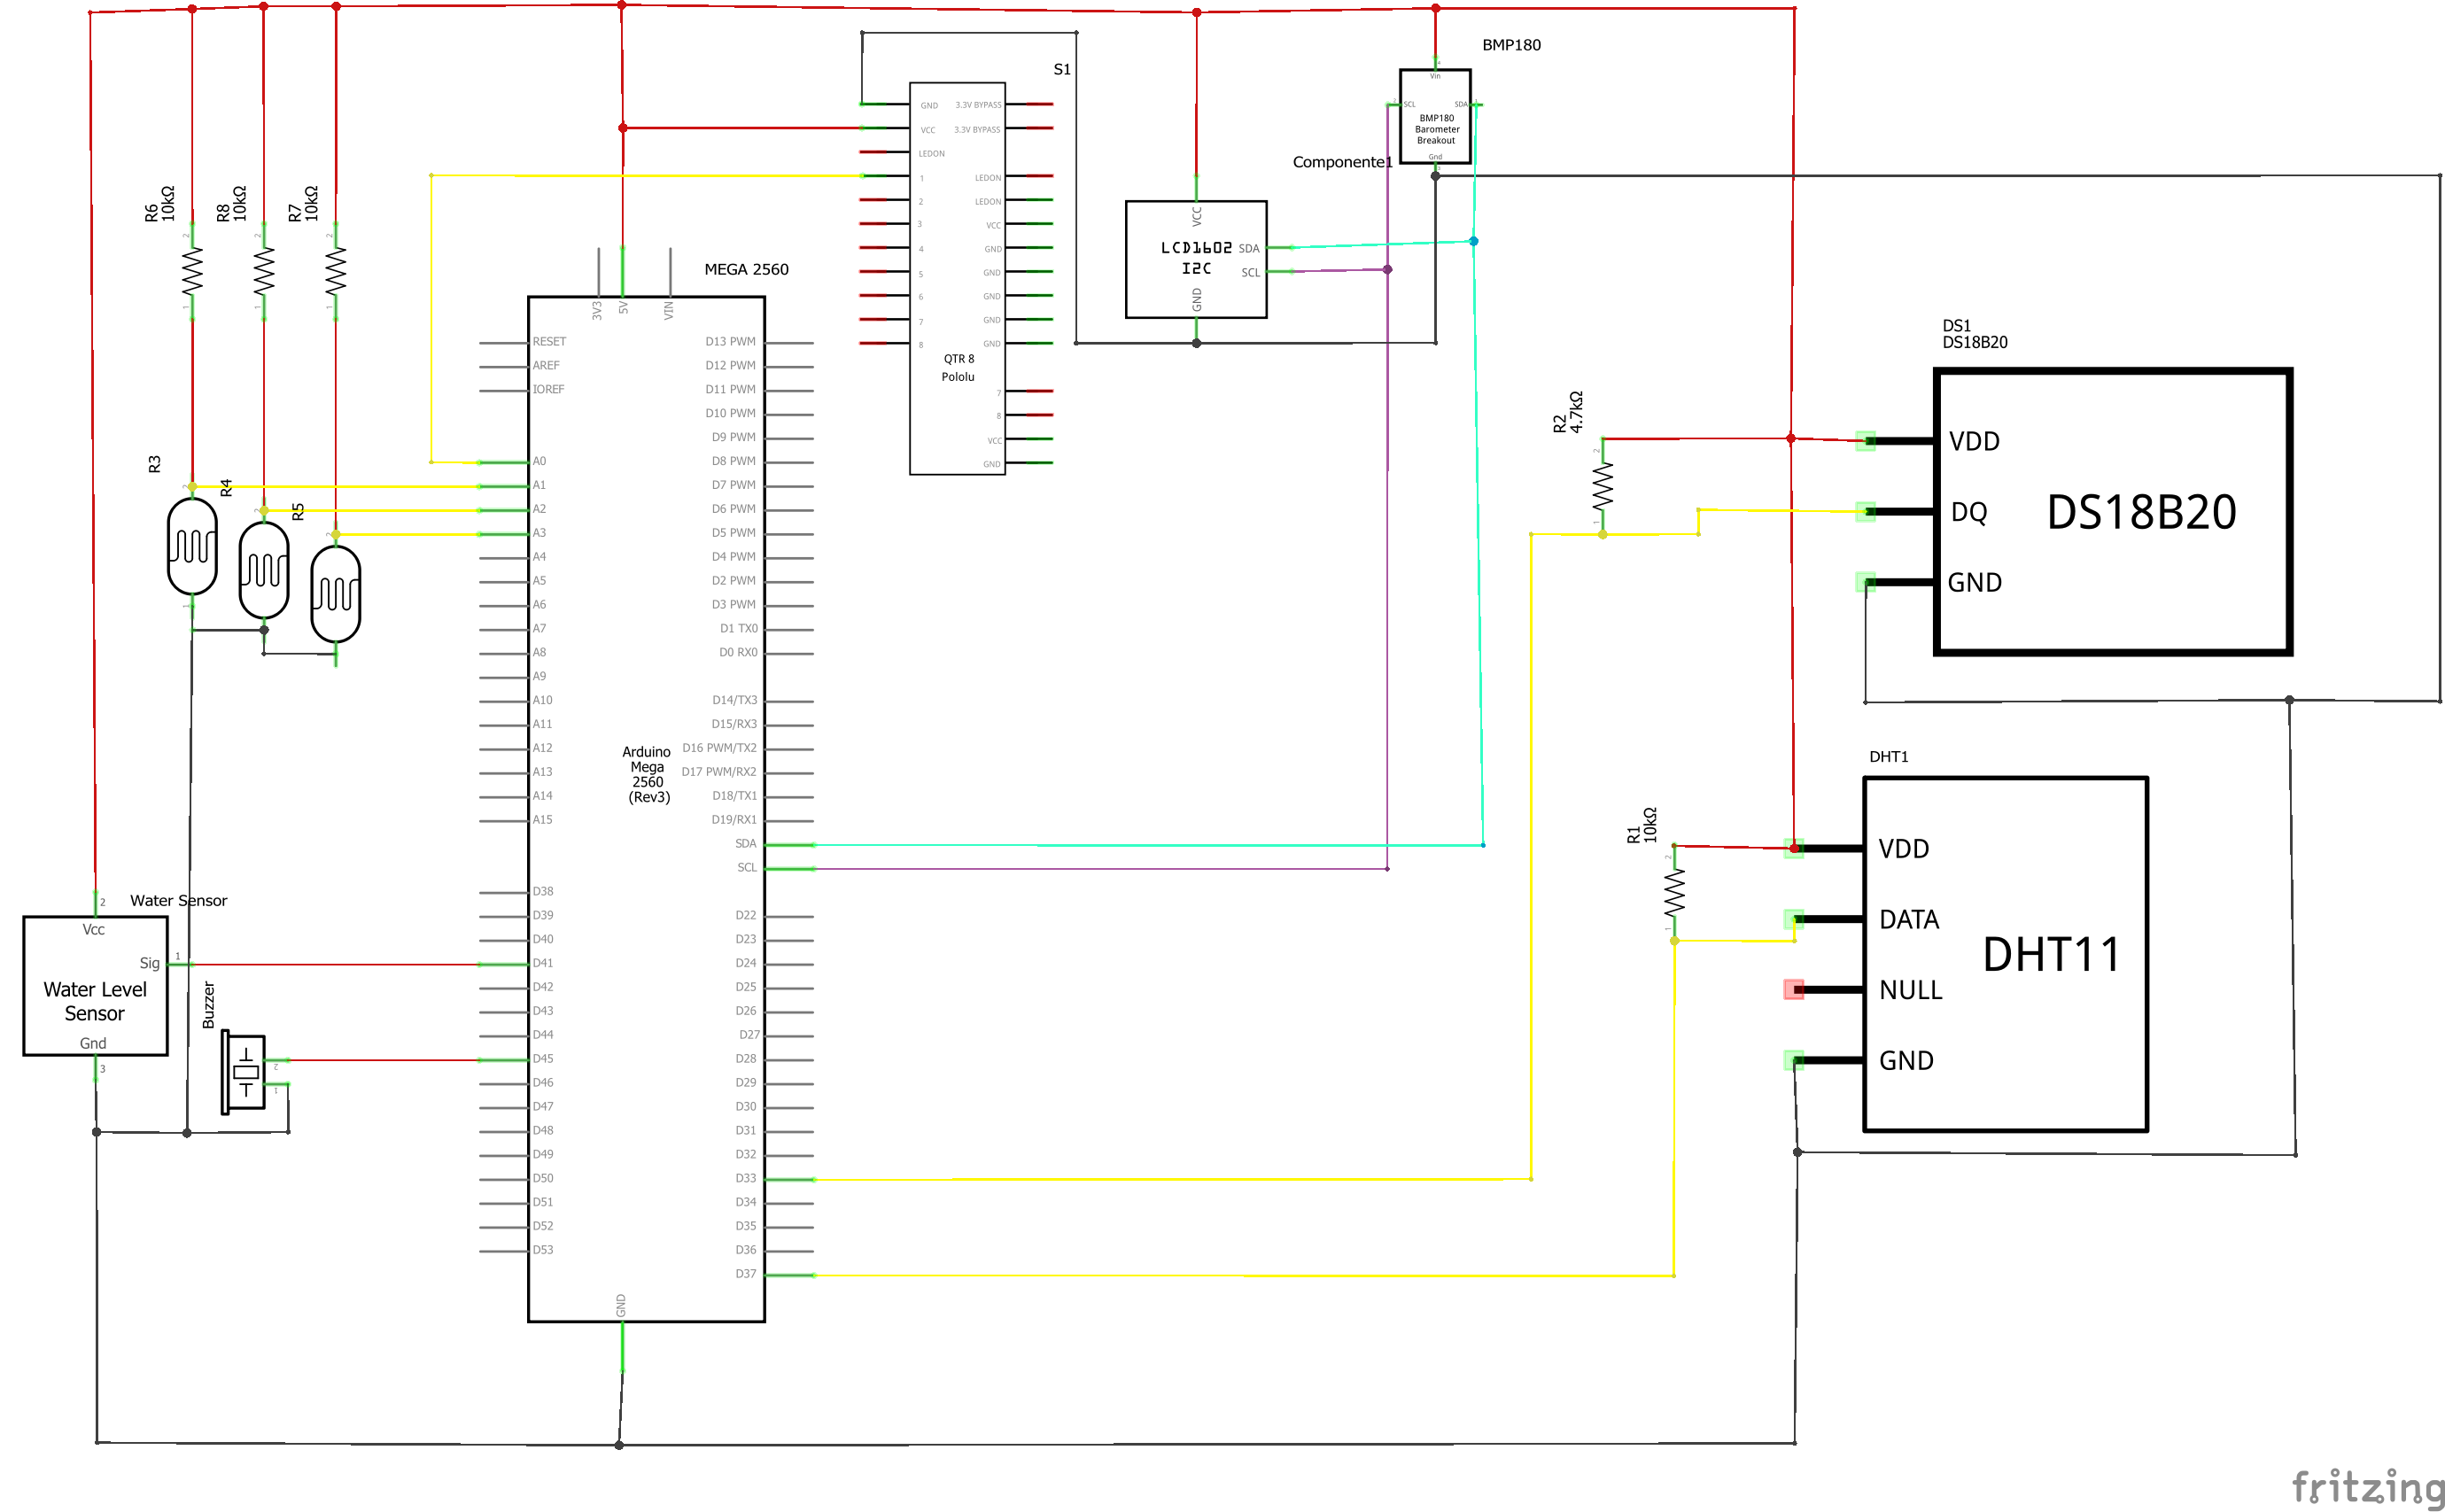
\includegraphics[width=\textwidth]{Prints/esquema.png}
\caption{Esquema do projecto}
\label{Rotulo}
\end{figure}

\newpage
Na imagem seguinte podemos ver o projecto totalmente finalizado.

\begin{figure} [!h]
\centering
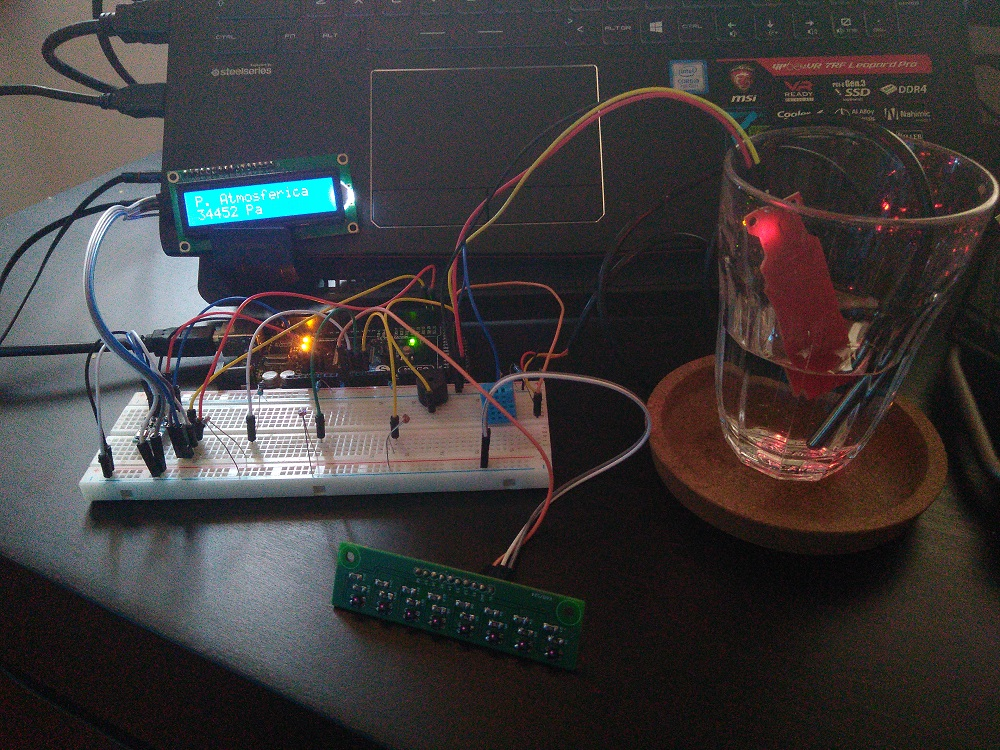
\includegraphics[width=\textwidth]{Prints/projecto.png}
\caption{Foto do projecto finalizado.}
\label{Rotulo}
\end{figure}



% Desenvolvimento
\chapter*{Desenvolvimento}
\addcontentsline{toc}{chapter}{Desenvolvimento}

Inicialmente decidimos que a nossa abordagem ao projecto seria começarmos por bare metal, testar todos os sensores e as ligações nesta metadologia de codigo e só depois passar a parte que iriamos recorrer ao sistema operativo FreeRTOS. \linebreak

Começamos por testar o sensor de temperatura DS18B20, para este recorremos a a biblioteca OneWire.h \cite{OneWire} para facilitar a leitura dos dados dos sensores. \cite{WaterproofDS18B20} \cite{sparkfunDS18B20}. De seguinda passamos ao sensor DHT11 que nos permite medir a pcertagem de humidade do ambiente e a temperatura. Para este recorremos a biblioteca DHT.h \cite{DHTadafruit}. \cite{DHT}. Depois passamos ao barómetro BMP180, este sensor permite-nos medir a pressão atmosferica, a temperatura e com a pressão atmosferica podemos calcular aproximadamente a altitude que encontra.  Para obter os valores recorremos a biblioteca  Wire.h  (nativa do arduino) e a  Adafruit\_BMP085.h \cite{bmpBiblio}. \cite{bmp}. Depois do circuito destes sensores montados e o codigo escrito, passamos a imprimir o valor deste na consola para verificar se estava tudo a funcionar correctamente. \linebreak

O proximo passo foi testar o sensor de detecção de água, este foi bastante simples tendo em conta que devolve um sinal HIGH (5V) caso seja encontrada água nos contactos do sensor. \cite{water}. Depois montamos os 3 LDR's que servem para determinar a posição do sol, este foram também bastaste simples tendo em conta que já tinhamos feito circuitos com a utilização de LDR's no decorrer da cadeira. Só tivemos que os ligar e determinar no codigo qual dos LDR's estava a obter um valor de resistencia mais baixo. \linebreak

Por fim faltava utilização de LED's infarvemelhos para ler a as rotações de um cata-vento, primeiro testamos utilizar simples LED's IR e contar as vezes que este era interrupido num certo periodo de tempo. Não obtimos sucesso, por isso recorremos ao sensor QTR-8RC mas utilizamos apenas um dos conjuntos de LED's. Para obter a leitura das Rotações por minuto fizemos uma função que durante 5 segundos consulta o valor obtido na porta analogica do LED receptor de 50 em 50 milisegundos. Caso este valor seja inferior ao do threshold definido (800) conta uma volta. Também tivemos que definir uma flag para evitar as mesmas leitura (caso o cata-vento estive-se parado). Para calcular um valor das rotações por minuto efectuamos uma regra de 3 simples para efectuar uma estimativa das rotações num minuto. \pagebreak

Como podemos verificar na imagem seguinte, estavamos a obter os valores dos sensores todos na consola.


\begin{figure} [!h]
\centering
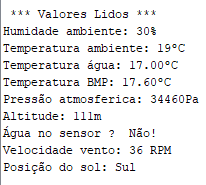
\includegraphics[width=50mm]{Prints/valores_consola.png}
\caption{Valores obtidos na consola do IDE.}
\label{Rotulo}
\end{figure}

O unico aspecto que nos faltava para terminar a implementação em bare metal era mostrar os valores dos sensores num LCD 16x2.




\clearpage



% Conclução
\chapter*{Conclusão}
\addcontentsline{toc}{chapter}{Conclusão}

Este trabalho permitiu-se aplicar os conhecimentos adquiridos durante o desenrolar da unidade curricular de Integração de Sistemas de Informação e explorar e desenvolver processos de interoperabilidade entre sistemas, assentes em serviços web. Uma das partes que correu mal no trabalho foi o uso da base de dados alojada no \textit{Azure} que por algum motivo não mantinha a ligação aberta quando a tentava usar no serviço. De qualquer forma acho que este trabalho foi um sucesso tendo conseguido alcançar os meus objetivos e ficando a conheçer mais sobre serviços RESTful.

% Bilbiografia
\begin{thebibliography}{2}

	\bibitem{OneWire}
	 PaulStoffregen. \emph{OneWire.h}.  06 Abril, 2018. 
	\url{https://github.com/PaulStoffregen/OneWire}


	\bibitem{WaterproofDS18B20}
	dfrobot. \emph{Waterproof DS18B20 Digital Temperature Sensor}.  06 Abril, 2018. 
	\url{https://github.com/PaulStoffregen/OneWire}


	\bibitem{sparkfunDS18B20}
	sparkfun. \emph{DS18B20}.  06 Abril, 2018. 
	\url{https://github.com/sparkfun/simple_sketches/blob/master/DS18B20/DS18B20.ino}

	\bibitem{DHTadafruit}
	 Adafruit. \emph{Adafruit Unified Sensor Driver.}  06 Abril, 2018. 
	\url{https://github.com/adafruit/Adafruit_Sensor}

	\bibitem{DHT}
	 lady ada. \emph{Connecting to a DHTxx Sensor.}  06 Abril, 2018. 
	\url{https://learn.adafruit.com/dht/connecting-to-a-dhtxx-sensor}


	\bibitem{bmpBiblio}
	Adafruit. \emph{A powerful but easy to use BMP085/BMP180 Library.}  06 Abril, 2018. 
	\url{https://github.com/adafruit/Adafruit-BMP085-Library}


	\bibitem{bmp}
	 Adilson Thomsen. \emph{Controlando temperatura e pressão com o BMP180.}  06 Abril, 2018. 
	\url{https://www.filipeflop.com/blog/temperatura-pressao-bmp180-arduino/}

	\bibitem{water}
	 tutorialspoint. \emph{Arduino - Water Detector / Sensor.}  20 Abril, 2018. 
	\url{https://www.tutorialspoint.com/arduino/arduino_water_detector_sensor.htm}





	

\end{thebibliography}
\addcontentsline{toc}{chapter}{Bibliografia}

\end{document}